% Pandoc/Quarto adapter for the unmodified IEEE Access 2026-05-13 class.
\documentclass{ieeeaccess}
\usepackage{amsmath,amssymb,amsfonts}
\usepackage{graphicx,textcomp,booktabs,array,multirow}
\usepackage[numbers,sort&compress]{natbib}
\usepackage[hidelinks]{hyperref}
\usepackage{bm}
\makeatletter
\AtBeginDocument{\DeclareMathVersion{bold}
\SetSymbolFont{operators}{bold}{T1}{times}{b}{n}
\SetSymbolFont{NewLetters}{bold}{T1}{times}{b}{it}
\SetMathAlphabet{\mathrm}{bold}{T1}{times}{b}{n}
\SetMathAlphabet{\mathit}{bold}{T1}{times}{b}{it}
\SetMathAlphabet{\mathbf}{bold}{T1}{times}{b}{n}
\SetMathAlphabet{\mathtt}{bold}{OT1}{pcr}{b}{n}
\SetSymbolFont{symbols}{bold}{OMS}{cmsy}{b}{n}
\renewcommand\boldmath{\@nomath\boldmath\mathversion{bold}}}
\makeatother
\providecommand{\tightlist}{\setlength{\itemsep}{0pt}\setlength{\parskip}{0pt}}
\providecommand{\pandocbounded}[1]{#1}
\makeatletter
\@ifpackageloaded{caption}{}{\usepackage{caption}}
\AtBeginDocument{%
\ifdefined\contentsname
  \renewcommand*\contentsname{Table of contents}
\else
  \newcommand\contentsname{Table of contents}
\fi
\ifdefined\listfigurename
  \renewcommand*\listfigurename{List of Figures}
\else
  \newcommand\listfigurename{List of Figures}
\fi
\ifdefined\listtablename
  \renewcommand*\listtablename{List of Tables}
\else
  \newcommand\listtablename{List of Tables}
\fi
\ifdefined\figurename
  \renewcommand*\figurename{Figure}
\else
  \newcommand\figurename{Figure}
\fi
\ifdefined\tablename
  \renewcommand*\tablename{Table}
\else
  \newcommand\tablename{Table}
\fi
}
\@ifpackageloaded{float}{}{\usepackage{float}}
\floatstyle{ruled}
\@ifundefined{c@chapter}{\newfloat{codelisting}{h}{lop}}{\newfloat{codelisting}{h}{lop}[chapter]}
\floatname{codelisting}{Listing}
\newcommand*\listoflistings{\listof{codelisting}{List of Listings}}
\makeatother
\makeatletter
\makeatother
\makeatletter
\@ifpackageloaded{caption}{}{\usepackage{caption}}
\@ifpackageloaded{subcaption}{}{\usepackage{subcaption}}
\makeatother
% Quarto loads caption/subcaption for cross references. Preserve the caption
% typography supplied by ieeeaccess.cls instead of caption's generic fallback.
\DeclareCaptionFont{accessfigure}{\figcapfont}
\DeclareCaptionFont{accessfigurelabel}{\color{accessblue}\figcapheadfont}
\DeclareCaptionFont{accesstable}{\tablecapfont}
\DeclareCaptionFont{accesstablelabel}{\color{accessblue}\tablecapheadfont}
\captionsetup[figure]{font=accessfigure,labelfont=accessfigurelabel,labelsep=period,justification=raggedright,singlelinecheck=false}
\captionsetup[table]{font=accesstable,labelfont=accesstablelabel,labelsep=period,justification=raggedright,singlelinecheck=false}
\AtBeginDocument{\renewcommand{\figurename}{FIGURE}\renewcommand{\tablename}{TABLE}}
\begin{document}
\vol{XX}
\year{XXXX}
\history{Manuscript prepared for review.}
\doi{To be assigned}
\title{Evaluation Pipeline Effects in Cross-Domain Deepfake Detection}
\author{\uppercase{Shiyu Chen}\authorrefmark{1}, AND
\uppercase{Kangbin Yim}\authorrefmark{2}}
\address[1]{Department of Software Convergence, Soonchunhyang University,
Asan 31538, Republic of Korea (e-mail: chen@sch.ac.kr)}
\address[2]{Department of Information Security, Soonchunhyang University,
Asan 31538, Republic of Korea (e-mail: yim@sch.ac.kr)}
\corresp{Corresponding author: Kangbin Yim (e-mail: yim@sch.ac.kr).}
\markboth{Chen and Yim: Evaluation Pipeline Effects in Deepfake
Detection}{Chen and Yim: Evaluation Pipeline Effects in Deepfake
Detection}
\begin{abstract}
Comparisons of deepfake detectors depend on the evaluation pipeline as
well as the learned model. We examine four sources of variation: face
preprocessing history, feature normalization at inference, video
grouping and score aggregation, and threshold transfer. Paired
experiments use three pretrained backbones, five training seeds for
scoring comparisons, and three seeds for preprocessing comparisons. With
identical frame features and classifier heads, inference normalization
decreases the area under the receiver operating characteristic curve for
all five DINOv2 models under mean-logit aggregation, but increases it
under mean-probability aggregation. Merging videos with matching
identifiers across forgery methods amplifies the latter gain from 0.90
to 3.41 percentage points while reducing absolute discrimination.
Preprocessing history also affects fixed deployment inputs: sequentially
processed training images reduce CLIP performance on DeepFakeDetection
by 1.58 percentage points on average, and paired comparisons quantify
changes in the gaps between backbones when test preprocessing changes.
Finally, CLIP achieves an area under the curve of 92.89 percent on a
fixed cross-domain test set while its source-calibrated threshold
misclassifies every real video. Calibration with twenty target real
videos excluded from testing raises balanced accuracy to 84.39 percent.
These controlled comparisons identify which pipeline operation changes
each conclusion and provide a reproducible basis for detector
comparison.
\end{abstract}
\begin{keywords}
cross-domain evaluation, deepfake detection, face preprocessing, feature
normalization, video aggregation
\end{keywords}
\titlepgskip=-21pt
\maketitle
\section{Introduction}\label{introduction}

Deepfake detection systems are often compared by transferring a detector
from one dataset to another and reporting video-level area under the
receiver operating characteristic curve (AUC). Such a comparison
combines several operations: constructing face images, selecting a model
checkpoint, transforming frame scores, defining video identities, and
choosing a deployment threshold. A change in any of these operations can
alter the measured result. Establishing where the change occurs is
therefore necessary before attributing a performance difference to a
detection method.

DeepfakeBench addresses comparability through unified data management,
detector implementations, and evaluation protocols
\citep{deepfakebench}. DF40 expands the range of forgery techniques and
evaluation settings \citep{df40}. These resources make systematic
comparisons possible, but a benchmark score still depends on the
concrete pipeline used in an experiment. For example, reprocessing an
already aligned face need not reproduce a face extracted directly from
the original frame. Similarly, averaging frame probabilities and
averaging frame logits need not preserve the same video ranking. An
incomplete video identifier can additionally combine outputs from
different forgery methods.

Pretrained visual encoders provide a useful setting in which to examine
these issues. CLIP, DINOv2, and EfficientNet learn representations under
different pretraining objectives \citep{clip, dinov2, efficientnet}.
When their output features are normalized only at inference, the
original classifier receives a different feature magnitude. Whether this
intervention improves cross-domain ranking depends on both the
classifier and the subsequent aggregation rule. A high AUC also leaves
open whether a threshold selected from source-domain real videos remains
usable after transfer.

We examine these dependencies through four paired questions. First, does
a complete preprocessing history affect a detector evaluated on an
identical deployment input, and does it change the response to test
preprocessing? Second, how does the AUC effect of inference-time
normalization depend on aggregation and its baseline? Third, can merging
video identities across forgery methods change the relative
normalization conclusion? Fourth, how do source and target real-video
calibration differ when evaluated on the same test videos? We hold the
relevant inputs or predictions fixed for each comparison. The
contribution is an empirical separation of these pipeline effects,
supported by saved predictions, explicit evaluation units, and
reproducible paired reductions.

\section{Related Work}\label{related-work}

\subsection{Datasets and evaluation
protocols}\label{datasets-and-evaluation-protocols}

FaceForensics++ (FF++) provides manipulated facial videos from four
methods and supports evaluations across compression settings
\citep{faceforensics}. Celeb-DF supplies a different collection of
realistic face forgeries \citep{celebdf}. DF40 generates a broader set
of manipulations across content sources \citep{df40}. We distinguish the
DF40 images generated from FF++ and Celeb-DF content from the original
videos in those datasets. Our scoring experiments use the released DF40
images; our preprocessing experiments reconstruct images from original
FF++ and DeepFakeDetection (DFD) videos. This distinction prevents a
cross-content experiment from being mistaken for evaluation on the
original Celeb-DF forgery collection.

DeepfakeBench identifies inconsistent inputs and evaluation settings as
obstacles to fair comparison \citep{deepfakebench}. Our experiments
extend this evaluation perspective by manipulating individual operations
on paired data. We retain the complete preprocessing trajectory, the
method component of a video identity, the order of aggregation and
probability conversion, and the source of calibration data. Each
comparison can consequently be linked to a specified operation rather
than to an unspecified end-to-end pipeline change.

\subsection{Visual representations and face
preprocessing}\label{visual-representations-and-face-preprocessing}

CLIP uses image--text supervision, DINOv2 uses self-supervised visual
learning, and EfficientNet uses compound scaling for convolutional
networks \citep{clip, dinov2, efficientnet}. We fine-tune their visual
encoders and a binary linear head. Our normalization comparison
preserves the fitted head, so it measures an inference intervention on
an existing classifier. It does not estimate the capacity of normalized
features after refitting a new head.

Face localization and alignment introduce another source of variation
before the encoder. RetinaFace predicts facial landmarks together with
face detections \citep{retinaface}. The dlib implementation combines a
histogram-of-oriented-gradients face detector with a 68-landmark
predictor and provides a face-chip alignment rule \citep{dlib}. We
compare two complete processing histories built from these components.
The experiment estimates their combined effect, including detection,
geometry, intermediate resolution, image content, and processing
failures; it does not assign that effect to a single component.

\section{Experimental Design}\label{experimental-design}

\subsection{Two complementary experiment
routes}\label{two-complementary-experiment-routes}

The scoring route, denoted D in the accompanying records, uses a fixed
21-method subset of DF40. It trains on FF++-content images (DF40-FF) and
evaluates transfer to Celeb-DF-content images (DF40-CDF). We save one
set of frame features and the original linear head for every selected
model. All inference and aggregation contrasts reuse those bytes. Five
formal training seeds, 7, 42, 123, 2026, and 3407, are used for each
backbone.

The preprocessing route, denoted H, uses FF++ c23 original videos for
training and source evaluation, and DFD original videos for transfer. It
constructs two processing histories from the same original frames and
trains a paired model for each history. The formal seeds are 7, 42, and
123. EfficientNet-B0 was evaluated first, and the same frozen cohorts
and paired design were then extended to CLIP and DINOv2 under the agreed
conditional expansion. All models receive \(224\times224\) images.

\subsection{Models, optimization, and checkpoint
selection}\label{models-optimization-and-checkpoint-selection}

We use OpenAI CLIP ViT-B/16, the official DINOv2 ViT-B/14 without
register tokens, and ImageNet-pretrained EfficientNet-B0. Their feature
dimensions are 512, 768, and 1280. The complete visual encoder and a new
two-output linear classifier are fine-tuned with cross-entropy. Learning
rates are \(10^{-5}\), \(5\times10^{-5}\), and \(10^{-4}\),
respectively. AdamW uses weight decay \(5\times10^{-4}\). Actual batch
size is 128, automatic mixed precision uses FP16, and gradient norm is
clipped at 1.0. We add no output-feature normalization during training;
each backbone retains its native normalization layers.

Training augmentation follows the fixed official DF40 implementation:
horizontal flipping, rotation within \(\pm10^{\circ}\), Gaussian blur
with kernel sizes 3--7, color transformations, and JPEG compression with
quality 40--100, with the corresponding random modules applied at
probability 0.5 and the original aspect-ratio resize step retained
\citep{df40code}. Input normalization matches each pretrained encoder.
Evaluation uses no random augmentation. The epoch schedule has one
configured warmup epoch followed by cosine decay; this configuration
reaches the initial learning rate in the first epoch.

An exponential moving average (EMA) with decay 0.999 is updated after
every successful optimizer update; buffers use the current model values.
The source validation metric is correct-video, mean-probability AUC
evaluated with EMA weights. In D, a checkpoint is selected by its own
source validation score, with patience five. In H, both histories are
evaluated on the same source B validation images, and the mean of their
AUCs selects one common epoch for the paired EMA checkpoints.

Independent development seeds 1007 and 1042 precede the formal seeds. D
development can use source validation and an isolated DF40-CDF
development set. We compare candidate budgets through the
source-selected checkpoint from each run and restart training when the
total cosine-schedule budget changes. Two- and five-epoch confirmation
runs select a two-epoch cap for CLIP and EfficientNet-B0. DINOv2 retains
a 30-epoch cap with source early stopping. The selected formal DINOv2
epochs are 9, 12, 21, 17, and 13; these differ from both the cap and the
development runs.

Figure~\ref{fig-development} shows the observed source and
target-development trajectories for the shared-budget development runs.
The two DINOv2 runs stop at epochs 27 and 25 and select source
checkpoints at 22 and 20, whereas their target-development maxima occur
much earlier. Thus, closeness between source and target preferred epochs
is an empirical question rather than an assumption of the protocol. The
curves are development evidence; no formal-test epoch curve is used for
checkpoint selection. Other budget-confirmation trajectories are
retained with the source data.

\begin{figure*}

\centering{

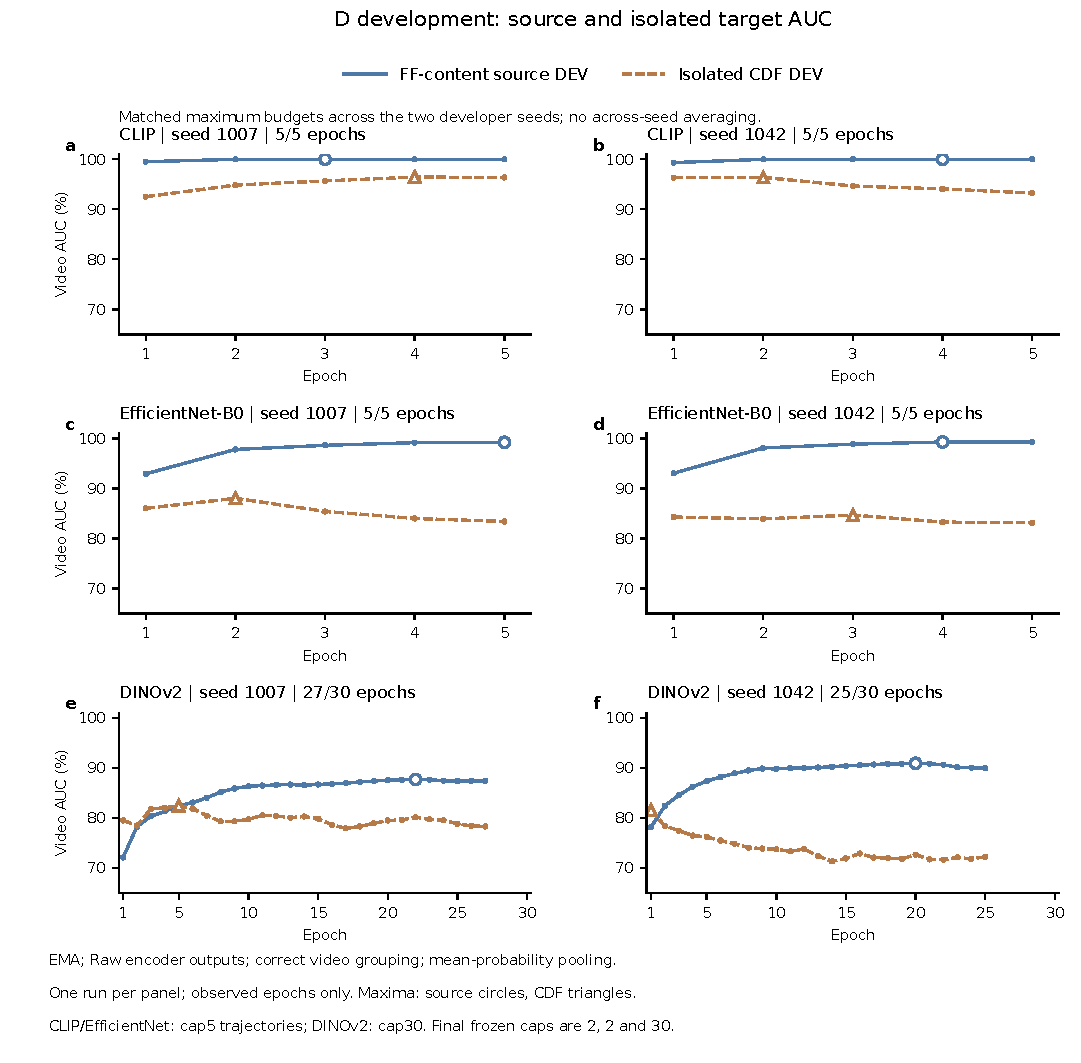
\includegraphics[width=1\linewidth,height=\textheight,keepaspectratio]{figures/development_auc.pdf}

}

\caption{\label{fig-development}Source and isolated target-development
AUC trajectories. Columns show CLIP, EfficientNet-B0, and DINOv2; rows
show development seeds 1007 and 1042. All curves use EMA weights, raw
features, correct video identities, and mean-probability aggregation.
The source is DF40-FF, and the target is the isolated DF40-CDF
development set. Each panel preserves all observed epochs of its
displayed run; companion source data contain the additional confirmation
budgets.}

\end{figure*}%

H uses a ten-epoch cap for all three backbones. CLIP retains its
original ten-epoch runs. Following inspection of the initial H results,
DINOv2 and EfficientNet-B0 were revised to exactly ten completed epochs,
replacing their original 60- and 15-epoch budgets. All twelve revised
models were restarted from public initialization, and their cosine
schedules were recomputed for ten epochs. The paired source criterion
selects the best EMA epoch within this window; patience is disabled for
the revised runs. Learning rate, optimizer, batch size, augmentation,
data, and pairing remain unchanged. This is a revision after initial
target results were available, rather than an originally target-blind
budget choice. DFD is not evaluated every epoch or used to select an
epoch within a revised run. DINOv2: paired epochs 10, 10, 10 for seeds
7, 42, and 123, respectively. All paired optima lie at the cap; a
source-validation plateau is not established within this window.
EfficientNet-B0: paired epochs 10, 10, 10 for seeds 7, 42, and 123,
respectively. All paired optima lie at the cap; a source-validation
plateau is not established within this window.

D has 799 batches per epoch and H has 185 per model, so epoch counts do
not denote equal optimization budgets between the routes. Formal
selected weights, successful updates, skipped mixed-precision updates,
and resolved recipes are recorded for all 33 models. Jobs run
independently on single V100 32 GB GPUs, with up to four concurrent GPU
jobs.

\subsection{Scoring data and frame
sampling}\label{scoring-data-and-frame-sampling}

The 21 methods comprise nine face-swapping methods---fsgan, faceswap,
simswap, inswap, blendface, uniface, mobileswap, e4s, and
facedancer---and twelve face-reenactment methods---fomm, facevid2vid,
wav2lip, MRAA, one\_shot\_free, pirender, tpsm, lia, danet, sadtalker,
mcnet, and hyperreenact. We use the released images and indices without
additional face detection or cropping. FF++ training source pairs are
partitioned into 306 training and 54 development pairs. Source
real-video calibration uses the official validation split, and source
testing uses the official test split. Eligibility and relationship
checks yield the counts in Table \ref{tab:d-cohorts}.

\begin{table}[t]
\centering
\caption{Frozen scoring cohorts after eligibility and relationship checks. The ranking cohort includes the 64 calibration real videos; threshold TEST excludes them.}
\label{tab:d-cohorts}
\setlength{\tabcolsep}{5pt}
\footnotesize
\begin{tabular}{lll}
\toprule
Role & Real videos & Fake videos \\
\midrule
DF40-FF training & 611 & 12,232 \\
DF40-FF development & 108 & 2,175 \\
Source real calibration & 140 & 0 \\
DF40-FF test & 140 & 2,884 \\
DF40-CDF development & 20 & 420 \\
DF40-CDF ranking & 157 & 12,037 \\
Target real calibration & 64 & 0 \\
DF40-CDF threshold test & 93 & 12,037 \\
\bottomrule
\end{tabular}
\end{table}

Every eligible natural video has eight fixed, distinct RGB frames.
Evaluation traverses all eight. Training contains 102,744
frame-association contributions; exact RGB duplicates are combined into
102,225 distinct inputs with their sampling masses added. The real class
receives probability mass 0.5, and each forgery method receives
\(0.5/21\), distributed over its videos and frames. Each epoch draws
102,272 inputs with replacement. Method balance therefore holds in
sampling expectation; realized counts need not be identical.

The target development set contains 20 real videos and 20 fake videos
per method. Isolation precedes prediction. Its relationship closure
includes known sources, exact RGB duplicates over all candidates,
cross-method matching names, and conservative identity-name proxies.
This excludes 890 related candidates from all formal target roles,
including 450 not used to score development. Development and formal
target roles have no video, relationship-group, or RGB intersection. The
full ranking cohort has 157 real videos, of which 64 also form the
target real-video calibration pool. Threshold comparisons exclude those
64 from the test cohort, leaving 93 real and 12,037 fake test videos.
All threshold policies use that identical reduced test cohort.

\subsection{Complete preprocessing
histories}\label{complete-preprocessing-histories}

FF++ c23 comprises 1,000 real videos and 1,000 fake videos from each of
Deepfakes, Face2Face, FaceSwap, and NeuralTextures. DFD contributes 363
real and 3,068 fake videos \citep{ffdata}. Before face processing, we
select eight distinct RGB mother frames using 32 fixed temporal
candidate positions per video and retain actual frame indices and
timestamps. A downstream processing failure never triggers replacement
with a different frame.

Pipeline A uses RetinaFace with MobileNet0.25, five facial landmarks,
detection score 0.6, and nonmaximum-suppression intersection over union
0.4 \citep{retinaface, retinaimplementation}. Detection has maximum
image side 1024. A least-squares, orientation-preserving similarity
transform aligns the five points to the ArcFace five-landmark template
defined at \(112\times112\) and scaled by three, yielding
\(336\times336\) pixels. Pipeline B uses the dlib HOG detector, one
upsampling step, a maximum detection side of 1024, and the 68-landmark
predictor \citep{dlib}. It computes geometry from the face-chip rule
with size 224 and padding 0.25, and renders the image using OpenCV
bicubic interpolation. A fixed rule resolves multiple detections using
face area, score, and coordinates.

The histories are original frame \(\rightarrow B\) and original frame
\(\rightarrow A\rightarrow B\), abbreviated B and AB. AB reads back the
persisted A PNG and runs the complete B detection, landmark estimation,
and alignment again. Zero padding and nearest-neighbor validity masks
are saved, and AB inherits invalid regions from A. The model sees RGB
only. Each eligible video requires successful processing of all eight
fixed frames and eight distinct final RGB images. Original selections,
PNGs, transforms, masks, and failure reasons are retained.

Training and development use the histories' common-success sets: 2,951
training videos (590 real, 2,361 fake) and 525 development videos (106
real, 419 fake). The models share initialization, seed, mother-frame
sampling, augmentation keys, and model-randomness synchronization during
paired updates. Real sampling mass is 0.5 and each fake method receives
0.125. Every epoch draws 23,680 frames with replacement. This design
keeps training membership and stochastic inputs paired across histories.

Model \(M_1\) is trained on B and \(M_2\) on AB. Their four evaluations
are \(H_{00}=M_1\rightarrow B\), \(H_{01}=M_1\rightarrow AB\),
\(H_{10}=M_2\rightarrow B\), and \(H_{11}=M_2\rightarrow AB\). The
deployment contrast is

\begin{equation}\protect\phantomsection\label{eq-fixed-b}{
\Delta_H=\operatorname{AUC}(H_{10})-\operatorname{AUC}(H_{00}),
}\end{equation}

evaluated on all B-success videos. The four-cell interaction is

\begin{equation}\protect\phantomsection\label{eq-history-interaction}{
\begin{aligned}
I_H={}&(\operatorname{AUC}(H_{11})-\operatorname{AUC}(H_{10}))\\
&-(\operatorname{AUC}(H_{01})-\operatorname{AUC}(H_{00})).
\end{aligned}
}\end{equation}

evaluated only on common-success videos. These contrasts retain their
own cohorts; we do not subtract AUCs across the two cohorts. Source test
membership is 139 real/558 fake for all B and 136/543 for common
success. DFD membership is 162/1,977 and 90/1,271, respectively.

\subsection{Inference normalization, aggregation, and video
identities}\label{inference-normalization-aggregation-and-video-identities}

Let \(h_i\) be a saved frame feature, \(W\) the two-output classifier
weights, and \(b\) its bias. The FP32 head is promoted to FP64 before
computing \(w=W_1-W_0\) and \(\beta=b_1-b_0\). The two frame margins are

\begin{equation}\protect\phantomsection\label{eq-margins}{
\begin{aligned}
z_i^{\mathrm{Raw}}&=w^\top h_i+\beta,\\
z_i^{\mathrm{L2}}&=w^\top\frac{h_i}{\max(\lVert h_i\rVert_2,10^{-12})}+\beta.
\end{aligned}
}\end{equation}

Features are exported in FP32. Both margins use the same saved features
and original head, and no classifier is refitted. For a video frame set
\(V\), we compare

\begin{equation}\protect\phantomsection\label{eq-aggregation}{
\begin{aligned}
S_{\mathrm{logit}}(V)&=\frac{1}{|V|}\sum_{i\in V}z_i,\\
S_{\mathrm{prob}}(V)&=\frac{1}{|V|}\sum_{i\in V}\sigma(z_i),
\end{aligned}
}\end{equation}

where \(\sigma\) is the sigmoid function. Applying \(\sigma\) after the
first average preserves its order in exact arithmetic. Averaging after
\(\sigma\) generally produces a different order. Numerical analyses
examine positive common scaling, common radii, Jensen gaps, frame
variance, probability endpoints, ties, and pairwise ranking credits,
using higher precision when needed to resolve endpoint ordering.

Correct grouping preserves domain, label, forgery method, and natural
video identifier. Collision grouping removes the method component and
merges matching identifiers within a domain and label. All \(8k\) frames
from \(k\) method-specific videos remain in the merged average; eight
frames are not resampled from that pool. Real videos remain individual
units. Source fake units consequently change from 2,884 videos to 280
collision groups; target fake units change from 12,037 to 1,830, with
140 and 157 real units unchanged. This is a controlled all-frame
grouping contrast, not a replay of a historical random draw of eight
frames from a merged folder.

The design has eight cells: Raw/L2 \(\times\) correct/collision
\(\times\) mean-logit/mean-probability. For each aggregation,
\(\Delta_{\mathrm{correct}}\) and \(\Delta_{\mathrm{collision}}\) are
the within-grouping AUC differences L2 minus Raw, and
\(I_G=\Delta_{\mathrm{collision}}-\Delta_{\mathrm{correct}}\). A
negative-to-positive reversal requires \(\Delta_{\mathrm{correct}}<0\)
and \(\Delta_{\mathrm{collision}}>0\) for the same seed. Positive
\(I_G\) alone does not meet this definition. Grouping changes the
statistical units and their weights, so the contrast diagnoses
sensitivity of the evaluation conclusion rather than improvement on an
identical set of video units.

For aggregation, we retain the exact identity
\(\Delta_{\mathrm{prob}}-\Delta_{\mathrm{logit}}=L_R-L_L\), where
\(L_R=\operatorname{AUC}(\mathrm{Raw,logit})-\operatorname{AUC}(\mathrm{Raw,prob})\)
and \(L_L\) is the corresponding L2 difference. A separate grouping
decomposition crosses natural-video versus group weighting with
member-score versus group-mean replacement. We average contributions
over the two operation orders and reconstruct original AUCs with exact
rational ranking credits. These are accounting decompositions of fixed
predictions, not training effects.

\subsection{Threshold transfer and statistical
reporting}\label{threshold-transfer-and-statistical-reporting}

For each of the four correctly grouped scores, we compare the default
threshold (0 for margins, 0.5 for probabilities), source-real
calibration, and target-real calibration. A calibrated threshold is the
smallest feasible value with empirical real-calibration false-positive
rate (FPR) at most 5 percent, using score \(\geq\) threshold as the fake
decision and fixed tie and boundary rules. Operating points use the
saved FP64 score space. Higher-precision ranking diagnostics do not
alter that deployed decision rule.

The main target budget is 20 real videos, with 10 and 40 as sensitivity
budgets. We draw 200 shared nested subsets from the 64-video target-real
pool; a budget of 80 is unavailable and remains missing. Every policy is
tested on the same 93 real/12,037 fake videos. We report FPR,
true-positive rate (TPR), balanced accuracy
\(\mathrm{BA}=(\mathrm{TPR}+1-\mathrm{FPR})/2\), and the underlying
false-positive and true-positive counts. Threshold changes leave scores
and AUC unchanged. For H, an additional source-calibrated analysis uses
139 real B calibration videos and transfers the same model-specific
threshold to both test histories.

We report all formal seeds and mean \(\pm\) sample standard deviation
(SD), with paired differences computed within each seed. D uses five
model seeds and H uses three. Calibration subsets are averaged within a
model before reporting variation across the five trained models. They
are not extra training replicates. Correct grouping also supports a
21-method equally weighted macro AUC; collision groups have no
single-method label. Per-method TPR and count reconstruction are
retained with the complete results.

Conditional group-bootstrap intervals use 2,000 shared draws and the
joint closure of source and collision relationships. We require at least
20 groups and no group larger than half the natural-video cohort, with
additional class- and method-level group checks. Unqualified intervals
remain missing rather than dropping difficult cases. DF40-CDF fakes form
one joint relationship group. DFD all-B real/fake groups number 12/16
and common-success groups 10/13. Target video-level population
confidence intervals are therefore unavailable under these rules. Seed
SD, calibration-subset variation, and conditional test-group uncertainty
are different quantities.

\section{Results}\label{results}

\subsection{Processing history changes coverage and image
content}\label{processing-history-changes-coverage-and-image-content}

The complete pipeline changes which videos can be evaluated
(Figure~\ref{fig-coverage}). On DFD, B retains 162 of 363 real videos
(44.63 percent) and 1,977 of 3,068 fake videos (64.44 percent). AB
retains 99 real and 1,362 fake videos (27.27 and 44.39 percent). Their
intersection contains 90 real and 1,271 fake videos. There are 778
B-only and 100 AB-only eligible videos. Thus, independently evaluating
each pipeline's success set would compare different video populations.
Our common-set crossing and fixed-B deployment contrast avoid that
ambiguity within their respective cohorts.

Requiring all eight prespecified frames matters for interpreting failure
rates. For DFD real videos, raw-frame B processing fails on 410 of 2,904
mother frames, but 201 of 363 videos fail the joint eight-frame
qualification. Six fake videos also lack enough distinct mother frames.
Failed processing is never repaired by choosing another frame. The mean
invalid image region on common-success source test videos changes from
0.0777 percent for B to 10.3214 percent for AB; corresponding DFD values
are 0.3089 and 10.0159 percent. These saved-mask measurements identify a
change in visible image support, without using the masks as model
inputs.

\begin{figure*}

\centering{

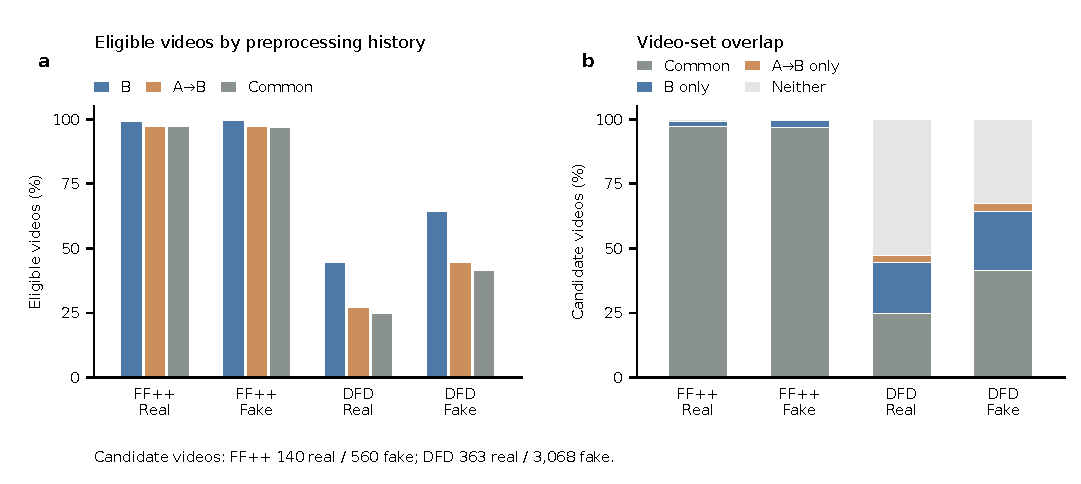
\includegraphics[width=1\linewidth,height=\textheight,keepaspectratio]{figures/preprocessing_coverage.pdf}

}

\caption{\label{fig-coverage}Video qualification and processing
coverage. The same frozen candidates and eight mother frames are used
for B and AB. Coverage is reported separately for source and target
classes; membership is partitioned into common success, B only, AB only,
and neither. All eight frames must succeed, and failures do not trigger
replacement. Counts enumerate the frozen candidate cohorts and have no
sampling error bars.}

\end{figure*}%

\subsection{Training history affects fixed deployment and responses to
test
processing}\label{training-history-affects-fixed-deployment-and-responses-to-test-processing}

On identical B deployment inputs, the training-history effect depends on
the backbone (Table \ref{tab:h-fixed}). For CLIP, AB training decreases
DFD AUC by \(1.5801\pm0.3008\) percentage points, with a decrease in all
three paired seeds. EfficientNet-B0 changes by \(+0.1382\pm0.6913\)
points, with 2 positive and 1 seed differences. DINOv2 changes by
\(+0.3814\pm3.8402\) points, with 1 positive and 2 negative paired
differences. These are raw-feature, mean-logit comparisons; their
uncertainty describes paired training variation on the fixed all-B
cohort.

\begin{table*}[t]
\centering
\caption{Fixed-B deployment AUC and paired training-history differences. Mean $\pm$ sample SD over three paired seeds; raw features and mean-logit aggregation.}
\label{tab:h-fixed}
\setlength{\tabcolsep}{5pt}
\footnotesize
\begin{tabular}{lllll}
\toprule
Backbone & Test domain & $M_1\to B$ AUC (\%) & $M_2\to B$ AUC (\%) & Paired difference (pp) \\
\midrule
CLIP & FF++ & $99.2913\pm0.1464$ & $99.0103\pm0.0356$ & $-0.2811\pm0.1477$ \\
CLIP & DFD & $97.1275\pm0.7723$ & $95.5474\pm0.9994$ & $-1.5801\pm0.3008$ \\
DINOv2 & FF++ & $66.1888\pm2.9850$ & $65.6782\pm0.7552$ & $-0.5106\pm3.0224$ \\
DINOv2 & DFD & $61.7020\pm4.6237$ & $62.0834\pm1.0222$ & $+0.3814\pm3.8402$ \\
EfficientNet-B0 & FF++ & $98.0532\pm0.0907$ & $98.0089\pm0.0250$ & $-0.0443\pm0.0775$ \\
EfficientNet-B0 & DFD & $93.6670\pm0.6867$ & $93.8052\pm0.9253$ & $+0.1382\pm0.6913$ \\
\bottomrule
\end{tabular}
\end{table*}

Changing test input history on the same common-success DFD videos
produces a training-history interaction (Figure~\ref{fig-history}). CLIP
gains \(0.4030\pm0.1204\) points from B-to-AB input switching for
\(M_1\), and \(1.7152\pm0.5063\) points for \(M_2\), giving interaction
\(+1.3122\pm0.3898\) points. EfficientNet-B0 changes by
\(-1.4990\pm0.3244\) and \(-0.0087\pm0.4545\) points for \(M_1\) and
\(M_2\), respectively, giving interaction \(+1.4902\pm0.6281\) points.
The revised DINOv2 interaction is \(+2.1523\pm1.8494\) points, with 3
positive and 0 negative seeds. The full four-cell AUCs and
mean-probability sensitivity contrasts are retained in the source data.
The fixed-B contrast and the interaction use different explicitly
defined cohorts.

The originally specified cross-backbone comparison is retained with the
revised weights. For AB-trained seed123 models on the same 90 real/1,271
fake DFD videos, CLIP scores 95.4507 percent under B and 97.3241 percent
under AB; EfficientNet-B0 scores 95.3842 and 95.2636 percent. The
CLIP-minus-EfficientNet gap changes from \(+0.0664\) to \(+2.0605\)
points. This specified M2 comparison has 0 strict point-estimate
reversals among three seeds. The complete family retains all 108
seed-level comparisons, including 0 strict point-estimate reversals.
This is a comparison of registered training recipes and pretrained
initializations, rather than an isolated architecture effect.

\begin{figure*}

\centering{

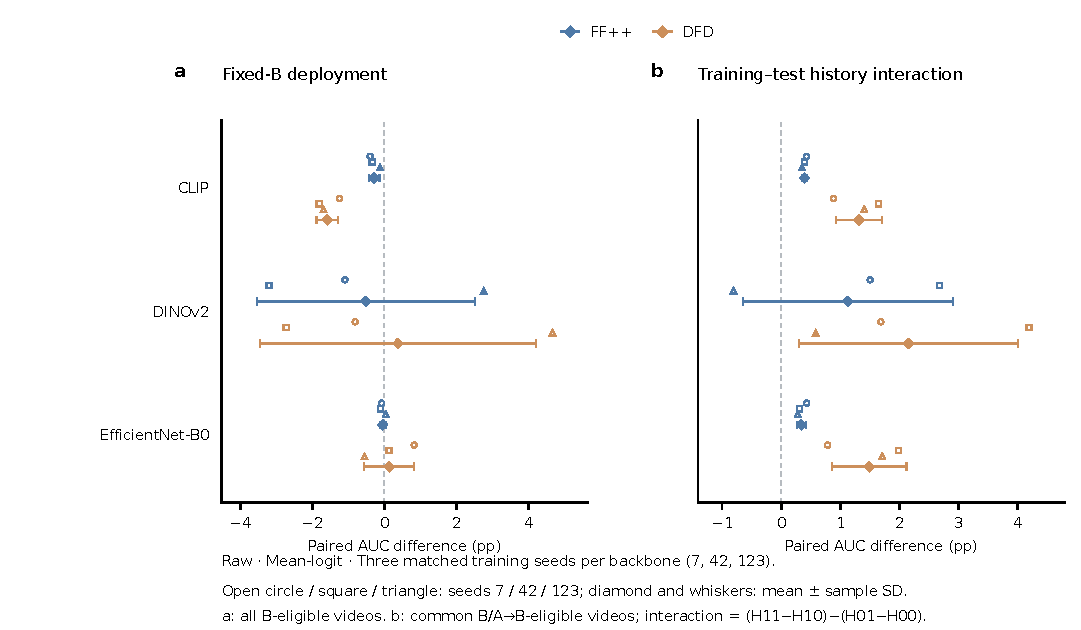
\includegraphics[width=1\linewidth,height=\textheight,keepaspectratio]{figures/preprocessing_effects.pdf}

}

\caption{\label{fig-history}Paired preprocessing-history effects. The
first panel shows AB-trained minus B-trained AUC on all B-success test
videos. The second shows the four-cell interaction on common-success
videos. All models use raw features and mean-logit aggregation. Markers
identify seeds 7, 42, and 123; diamonds and bars show the mean and
sample SD of within-seed differences. Each panel retains its own fixed
video cohort. DINOv2 and EfficientNet-B0 use the revised ten-epoch runs;
all backbones have a ten-epoch cap.}

\end{figure*}%

\subsection{Normalization conclusions depend on aggregation and video
units}\label{normalization-conclusions-depend-on-aggregation-and-video-units}

Under correct target-video grouping, mean-logit inference normalization
has a near-zero average effect for CLIP and a negative average effect
for DINOv2 and EfficientNet-B0. Mean-probability aggregation instead
yields positive average differences for all three, with different seed
consistency (Table \ref{tab:scoring}). In particular, every DINOv2 seed
decreases under mean-logit and increases under mean-probability. Under
mean-probability, CLIP improves in all five seeds and EfficientNet-B0 in
two. Aggregation can therefore change the direction of the fixed-head
normalization comparison even when video identities are correct.

\begin{table*}[t]
\centering
\caption{Complete target scoring design. AUC values show five-model mean $\pm$ sample SD. Differences are L2 minus Raw under the same grouping and aggregation.}
\label{tab:scoring}
\setlength{\tabcolsep}{5pt}
\footnotesize
\begin{tabular}{llllll}
\toprule
Backbone & Grouping & Aggregation & Raw AUC (\%) & L2 AUC (\%) & Mean difference (pp) \\
\midrule
CLIP & correct & mean-logit & $92.3864\pm0.9960$ & $92.3944\pm1.0555$ & $+0.0080$ \\
CLIP & correct & mean-probability & $91.5098\pm0.9230$ & $92.3840\pm1.0532$ & $+0.8742$ \\
CLIP & collision & mean-logit & $82.1421\pm1.3686$ & $82.4942\pm1.5205$ & $+0.3521$ \\
CLIP & collision & mean-probability & $80.3321\pm1.4079$ & $82.4873\pm1.5214$ & $+2.1552$ \\
DINOv2 & correct & mean-logit & $83.1673\pm1.4779$ & $83.0218\pm1.4983$ & $-0.1455$ \\
DINOv2 & correct & mean-probability & $82.1168\pm1.5947$ & $83.0163\pm1.4989$ & $+0.8996$ \\
DINOv2 & collision & mean-logit & $73.0197\pm2.1981$ & $72.1873\pm2.1307$ & $-0.8323$ \\
DINOv2 & collision & mean-probability & $68.7556\pm1.7740$ & $72.1652\pm2.1312$ & $+3.4096$ \\
EfficientNet-B0 & correct & mean-logit & $86.2212\pm0.8871$ & $85.9980\pm0.9630$ & $-0.2233$ \\
EfficientNet-B0 & correct & mean-probability & $85.9589\pm0.9338$ & $85.9960\pm0.9641$ & $+0.0371$ \\
EfficientNet-B0 & collision & mean-logit & $75.2114\pm0.5174$ & $74.4609\pm0.5067$ & $-0.7505$ \\
EfficientNet-B0 & collision & mean-probability & $74.0654\pm0.6871$ & $74.4497\pm0.5103$ & $+0.3843$ \\
\bottomrule
\end{tabular}
\end{table*}

Collision grouping reduces absolute AUC for both Raw and L2 across all
15 models, yet enlarges the mean-probability normalization gain
(Figure~\ref{fig-scoring}). Mean gains change from 0.8742 to 2.1552
points for CLIP, from 0.8996 to 3.4096 for DINOv2, and from 0.0371 to
0.3843 for EfficientNet-B0. This amplification should not be interpreted
as better detection: the collision-group absolute AUCs are lower. The
denominator of AUC is a set of real--fake ranking pairs, not a
class-balanced accuracy calculation, so bringing fake counts closer to
real counts is not by itself an explanation.

Under the strict negative-to-positive definition, CLIP mean-logit
reverses for one of five target seeds and EfficientNet-B0
mean-probability for three of five. DINOv2 has no such reversal under
either aggregation. EfficientNet-B0 mean-logit additionally has one
reversal in the opposite direction. None of the six target
backbone-by-aggregation five-seed mean contrasts changes from a negative
correct-grouping difference to a positive collision-grouping difference.
Seed-level reversals, positive interactions, and mean-level reversals
are consequently separate results.

Using Raw mean-logit as a common reference, correct-grouping L2
mean-probability differences are \(-0.0025\pm0.4511\),
\(-0.1509\pm0.0831\), and \(-0.2252\pm0.2374\) points for CLIP, DINOv2,
and EfficientNet-B0. The apparent positive differences against Raw
mean-probability therefore depend on that specific comparator. Saved
aggregation identities and ranking ledgers reconstruct the original
AUCs; 360 numerical negative controls preserve order. The separate
grouping decomposition reconstructs 120 cells and 60 interactions by
accounting for weight changes and score averaging. These checks quantify
how the evaluation changes without reducing all effects to sigmoid
saturation alone.

\begin{figure*}

\centering{

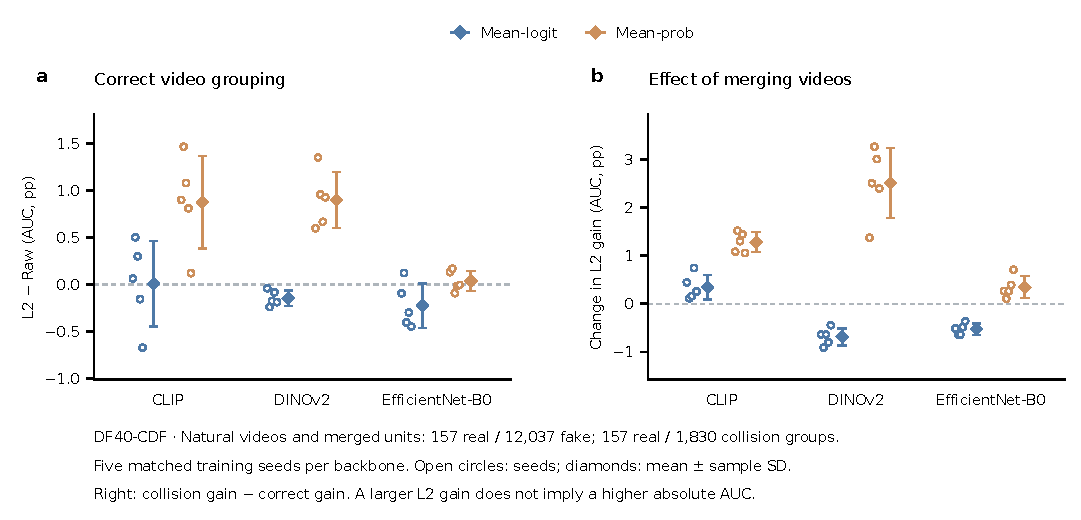
\includegraphics[width=1\linewidth,height=\textheight,keepaspectratio]{figures/normalization_grouping.pdf}

}

\caption{\label{fig-scoring}Normalization and grouping effects on
DF40-CDF. The first panel shows L2 minus Raw AUC with correct
natural-video identities. The second shows the collision-grouping
normalization gain minus the correct-grouping gain. Both aggregations
are retained. Open markers identify five formal training seeds, and
diamonds and bars show paired means and sample SD. Correct grouping
contains 157 real and 12,037 fake natural videos; collision grouping
contains 157 real and 1,830 merged fake units, retaining all eight
frames per constituent video. Positive interaction is distinct from a
direction reversal.}

\end{figure*}%

\subsection{High AUC can coexist with unusable source
thresholds}\label{high-auc-can-coexist-with-unusable-source-thresholds}

Source-real calibration for CLIP classifies every target test video as
fake under all four scoring choices and all five models. FPR and TPR are
both 100 percent and BA is 50 percent, despite high AUC on the same
videos. EfficientNet-B0 also has a high transferred-source FPR. DINOv2
has lower FPR together with lower recall. Table \ref{tab:operating}
gives the raw mean-logit comparison on the identical 93 real/12,037 fake
test cohort.

\begin{table*}[t]
\centering
\caption{Raw mean-logit operating points on the same 93 real and 12,037 fake target test videos. Target subset results are averaged within each model before computing five-model mean and sample SD.}
\label{tab:operating}
\setlength{\tabcolsep}{5pt}
\footnotesize
\begin{tabular}{llllll}
\toprule
Backbone & Calibration & Same-TEST AUC (\%) & FPR (\%) & TPR (\%) & BA (\%) \\
\midrule
CLIP & Source real & $92.8921\pm1.0313$ & $100.0000\pm0.0000$ & $100.0000\pm0.0000$ & $50.0000\pm0.0000$ \\
CLIP & Target real, $n=20$ & $92.8921\pm1.0313$ & $8.3333\pm1.9112$ & $77.1127\pm2.4273$ & $84.3897\pm1.3650$ \\
DINOv2 & Source real & $84.2911\pm1.3927$ & $8.3871\pm2.2036$ & $58.6641\pm3.3408$ & $75.1385\pm1.8493$ \\
DINOv2 & Target real, $n=20$ & $84.2911\pm1.3927$ & $7.2957\pm0.4982$ & $56.2656\pm3.1649$ & $74.4850\pm1.5989$ \\
EfficientNet-B0 & Source real & $87.0721\pm0.9020$ & $87.0968\pm5.5353$ & $99.0214\pm0.3731$ & $55.9623\pm2.5821$ \\
EfficientNet-B0 & Target real, $n=20$ & $87.0721\pm0.9020$ & $6.3688\pm1.4775$ & $58.6404\pm3.0616$ & $76.1358\pm1.2080$ \\
\bottomrule
\end{tabular}
\end{table*}

Twenty target-real calibration videos increase CLIP and EfficientNet-B0
average BA under all four scoring choices, but decrease DINOv2 average
BA under all four (Figure~\ref{fig-operating}). For raw mean-logit
scores, target-minus-source BA differences are \(+34.3897\pm1.3650\),
\(-0.6536\pm0.9560\), and \(+20.1735\pm3.5265\) points, respectively.
DINOv2's lower FPR is accompanied by lower TPR, so FPR alone would give
an incomplete account of calibration value.

Calibration uses only real videos at the threshold-estimation stage. D
model development has previously used both real and fake labels from the
isolated target development set; we do not describe the complete
development process as target-label-free. The 200 calibration subsets
are averaged within a model, and each model's 2,408 valid operating
points are independently reconstructed from counts. Budgets 10 and 40,
default thresholds, unavailable-budget records, and method-level TPRs
accompany the primary results. A finite real-calibration subset does not
guarantee a population FPR of five percent.

\begin{figure*}

\centering{

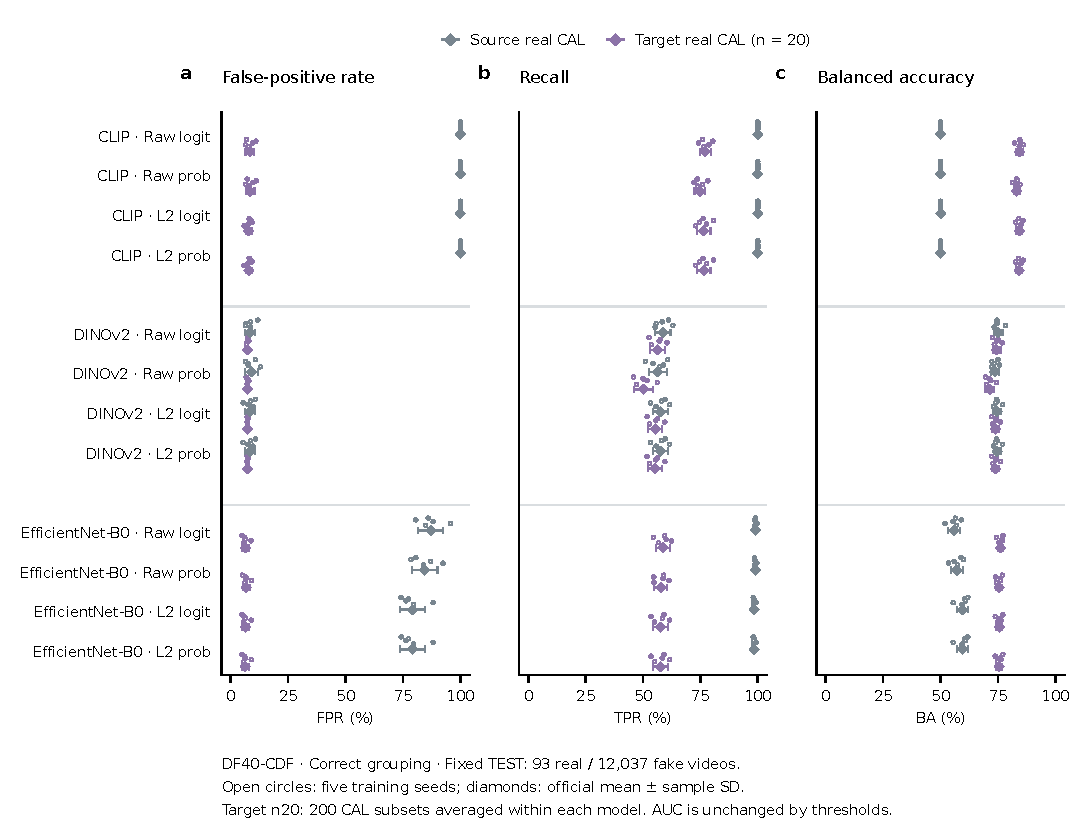
\includegraphics[width=1\linewidth,height=\textheight,keepaspectratio]{figures/operating_points.pdf}

}

\caption{\label{fig-operating}Transferred operating points under
source-real and target-real calibration. Panels show false-positive
rate, true-positive rate, and balanced accuracy for the four
correct-grouping scores. Open markers denote the five formal models.
Diamonds and error bars summarize model means and sample SD; each model
first averages its 200 target-calibration subsets. All policies use the
same fixed test videos, and threshold changes leave AUC unchanged.}

\end{figure*}%

\section{Discussion}\label{discussion}

These comparisons show that a detector's reported performance is
conditional on several distinct pipeline choices. Complete preprocessing
history changes input content and eligibility. Aggregation changes how
frame margins become video scores. Grouping changes both the comparison
units and their relative weight. Calibration changes decisions at a
fixed score distribution. Keeping these operations explicit extends the
unified-evaluation perspective of DeepfakeBench and the multi-method
scope of DF40 into paired, operation-specific evidence
\citep{deepfakebench, df40}.

The normalization result is particularly dependent on its baseline. The
head is trained on raw features, and normalizing each frame changes the
magnitude delivered to that fitted head. Applying sigmoid before
averaging further changes the contribution of frame margins. The DINOv2
sign change between aggregation rules and the common Raw mean-logit
reference establish why the same inference intervention can look
beneficial under one comparator and unhelpful under another. Saturated
probabilities, frame heterogeneity, and unequal norm scaling are related
but distinct possibilities. The numerical ledgers and controls constrain
their contributions without establishing a single universal saturation
mechanism. Refitting a head on normalized representations would address
a different question.

Collision grouping creates another form of evaluation sensitivity. AUC
averages ranking credit over real--fake pairs. Merging several
method-specific videos replaces multiple fake scores by a group score
and gives groups with different member counts equal evaluation mass.
Both the scores and their weighting change. This can enlarge the
difference between Raw and L2 even when both absolute AUCs decrease, as
observed here. Saving method-qualified natural identities, absolute
scores, paired gains, and reversal frequencies makes these
interpretations distinguishable. A claim that all three backbones
exhibit the same negative-to-positive reversal is unsupported by the
completed seed-level results.

The preprocessing experiment identifies a complementary input-side
effect. An identical final resolution does not imply identical image
content: detecting and aligning again after A changes geometry, visible
regions, and which videos survive. Testing both models on the same B
deployment data identifies the training-history contrast within that
cohort; crossing histories on the common-success set identifies a
different interaction. The cross-backbone comparisons quantify how
preprocessing changes between-model performance gaps under registered
recipes. Under the revised ten-epoch recipe, the B-trained DINOv2
source-test AUC is 66.1888 percent; the comparison therefore concerns
these fitted detectors, including their achieved source learning.
Component-wise attribution would require fixing all but one of
detection, landmarks, crop extent, interpolation, and intermediate
resolution.

Ranking and operating performance also require separate interpretation.
Any common strictly increasing score transform preserves exact ranking
but can change predictions at a fixed numerical threshold. CLIP's high
target AUC and complete source-threshold failure provide an empirical
example of this distinction. Target-real calibration repositions the
operating point, but its value depends on the existing threshold and the
associated recall tradeoff. DINOv2 shows why lower false alarms alone do
not establish higher balanced accuracy. Calibration-data provenance
belongs in a transfer evaluation alongside AUC.

The statistical scope follows the experimental units. Seed SD describes
training variability on frozen videos, and calibration-subset variation
describes threshold estimation from one real-video pool. Neither
substitutes for uncertainty across independent source identities. The
relationship closure prevents a defensible target group-bootstrap
interval under our reporting criteria, so target effects remain
descriptive paired estimates with explicit seed variation. Preprocessing
AUCs are additionally conditional on successful processing. Reporting
candidate denominators and failure reasons is necessary when applying
these conclusions to another deployment population.

\section{Conclusion}\label{conclusion}

Paired experiments separate the effects of preprocessing history,
feature normalization, video aggregation, and threshold transfer in
cross-domain deepfake detection. The measured normalization gain changes
with its aggregation baseline and can be amplified by erroneous video
merging. Complete preprocessing histories alter performance on identical
deployment inputs and alter between-backbone AUC gaps. High
discrimination can coexist with an unusable source-calibrated threshold.
Recording these conditions, their evaluation units, and their paired
predictions supports reproducible performance comparisons within the
tested datasets and training recipes.

\section*{Data and Code Availability}\label{data-and-code-availability}
\addcontentsline{toc}{section}{Data and Code Availability}

Original videos and released face images are accessed through the
official FF++, DFD, and DF40 resources \citep{ffdata, df40code}. Their
redistribution conditions continue to apply. Training and evaluation
code is available in the
\href{https://github.com/xiaotubaobiu/Disentangling-Angular-Norm-Deepfake-Detection}{project
repository}. The archived execution commit and the revised fixed-budget
implementation are identified separately in the accompanying provenance
records. Frozen splits, processing counts, complete seed-level tables,
figure source data, and verification receipts accompany this manuscript
in the local evidence archive. Checkpoints, FP32 features, original
heads, and per-video scores are retained there for recomputation.

\section*{Acknowledgment}\label{acknowledgment}
\addcontentsline{toc}{section}{Acknowledgment}

{[}AUTHOR INPUT REQUIRED: Funding and grant information.{]}

{[}AUTHOR INPUT REQUIRED: Title, venue, year, and publication status of
the accepted conference predecessor, its citation, and a concise account
of the journal extension. Proceedings details are pending.{]}

OpenAI Codex assisted with experimental code revision, numerical checks,
figure preparation, and drafting and translation of the abstract and
Sections I--VI. This draft and its disclosure require final review by
the named human authors before submission.
\bibliographystyle{IEEEtran}
\bibliography{references.bib}
\begin{IEEEbiographynophoto}{Shiyu Chen}
is with the Department of Software Convergence, Soonchunhyang University, Asan, Republic of Korea. [AUTHOR INPUT REQUIRED: academic background, research interests, and approved biography.]
\end{IEEEbiographynophoto}
\begin{IEEEbiographynophoto}{Kangbin Yim}
is with the Department of Information Security, Soonchunhyang University, Asan, Republic of Korea. [AUTHOR INPUT REQUIRED: academic background, research interests, and approved biography.]
\end{IEEEbiographynophoto}
\EOD
\end{document}
